%!TEX root = ../thesis.tex

\chapter{Eigener Ansatz} % (fold)
\label{cha:eigener_ansatz}


\begin{itemize}
    \item Probleme und deren Lösung während der Umsetzung
    \item Beispiel: Zugriff auf Moodle über Webservice
\end{itemize}


\todo[inline]{Auch begründen warum die Verwendung von Ontologien und nicht bspw. die Entwicklung eines XML Schemas (alternativ bei der Analyse Kap. 3.2)}

\section{Social Online Community Connectors} % (fold)
\label{sec:social_online_community_connectors}

\subsection{Datenformat} % (fold)
\label{sub:datenformat}

% subsection datenformat (end)

\subsection{Konfiguration} % (fold)
\label{sub:konfiguration}

\todo[inline]{Keine Erzählung nach dem Motto: erst haben wir das gemacht und dann gemerkt dass das nicht so toll war. Lieber begründen warum man das System so oder so konzipiert.}


Dass ein Connector funktionieren kann, muss er von außen mit Informationen zugeführt bekommen welche er zum Betrieb braucht. Die sind zum Beispiel Informationen zu Benutzerkonten oder Parameter für die verwendete API. Da einige dieser Informationen werden nicht nur von einen Connector benutzt werden, ist es sinnvoll diese zusammen an einen Ort zu speichern und wiederverwenden zu können. Die wichtigsten Informationen für die Konfiguration der Connectoren stellen die Benutzerkonten dar. Sie enthalten unter anderem die Informationen um Zugriff auf die einzelnen APIs zu erhalten. Da die Benutzerkonten wie im Abschnitt \ref{sub:datenformat} beschrieben im FOAF Format in einen Triplestore gespeichert werden, stellt es sich als Vorteil heraus die übrigen Informationen ebenfalls dort zu speichern und mit den schon vorhandenen zu verbinden. 

\medskip

Aus diesem Grund wurde für Konfiguration eines Connectors die \emph{Connector Config Ontology} entwickelt. Diese Ontologie ist sehr einfach gehalten und baut auf schon vorhandenen Ontologien auf. Zusätzlich musste die SIOC Ontologie so erweitert werden, dass die Integration von Autorisierungs- und Authentifizierungsinformationen möglich war. 

\subsubsection{Connector Config Ontologie} % (fold)
\label{ssub:connector_config_ontologie}

Abbildung \ref{fig:uebersicht_conector_cfg} zeigt die entwickelte Connector Con
 Ontologie. Sie besteht aus einer einzigen Klasse \texttt{ConnectorConfig} und vier Eigenschaften.

\medskip

\begin{figure}[ht]
    \centering
    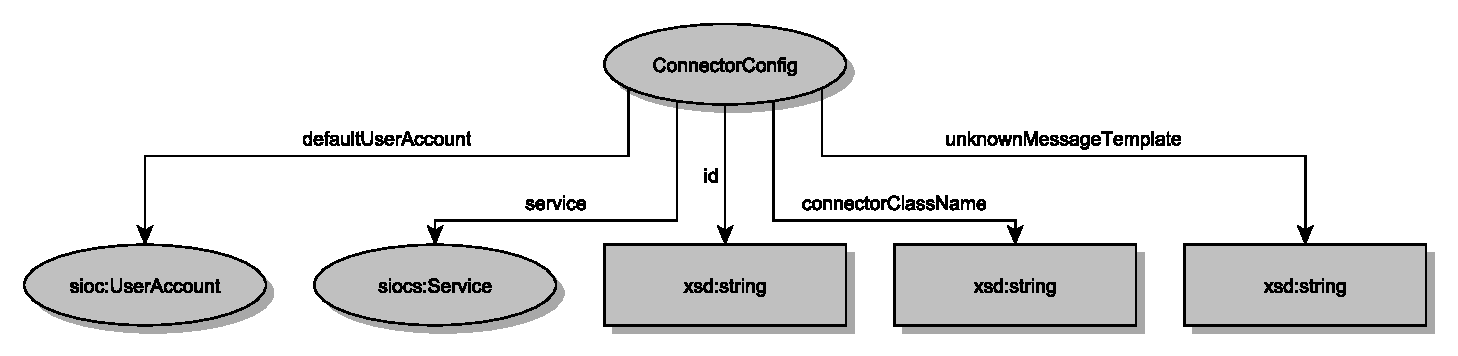
\includegraphics[
        width=\textwidth,
        keepaspectratio=true
    ]{assets/images/connector_config_ontology}
    \caption{Connector Config Ontology}
    \label{fig:uebersicht_conector_cfg}
\end{figure}

% subsubsection connector_config_ontology (end)
Jeder Connector erhält einen eindeutigen \texttt{id} zugewiesen, um jeden dieser Connectoren eindeutig identifizieren zu können. Die Eigenschaft \texttt{connectorClassName} beschreibt den vollständigen Klassennamen des beschriebenen Connector. Diese wird für das laden der richtigen Implementierung benötigt. Für die Nutzung einiger APIs müssen bestimmte Parameter angegeben werden. Dies könnte zum Beispiel die genau Adresse des Dienstes sein. Hierzu wird auf die schon Bestehende SIOC Services Ontologie zurückgegriffen. Diese stellt eine Klasse \emph{Service} zur Verfügung und mittels der Eigenschaft \texttt{service} kann ein solcher Service einem Connector zugewiesen werden. Der genaue Aufbau eines solchen Services wird im Abschnitt \ref{ssub:services} dargestellt. Die letzte Information für die Konfiguration eins Connectors ist eine vordefinierter Benutzer (im Folgenden Defaultuser genannt) und wird mit der Eigenschaft \texttt{defaultUserAccount} festgelegt. Dieser Defaultuser erfüllt im Großen und Ganzen zwei Aufgaben. Als Erstes wird er für lesende Zugriffe der API auf den verwendeten Dienst genutzt. Hierzu ist ein einzelnes Benutzerkonto vollkommen ausreichend, da nur die gelesenen Daten wichtig sind und nicht von welchen Konto sie kommen.Die zweite Aufgabe bezieht sich auf das stellvertretende Schreiben einzelner Benutzer. Nicht immer werden die dazu notwendigen Daten von den Benutzer zur Verfügung gestellt oder sind unbekannt. In diesem Fall wird der Defaultuser genutzt und der Beitrag mit einem Vermerk zum original Autor über diesen geschrieben.


\subsubsection{Services} % (fold)
\label{ssub:services}

Wie eben schon beschrieben, existiert für SIOC ein Modul zur einfachen Modellierung von Diensten auf semantischer Ebene. Kernstück dieses Moduls ist die Klasse Service, wie auf Abbildung \ref{fig:uebersicht_sioc_services} zu sehen ist. Mit dieser Klasse kann durch eine Hand voll Eigenschaften ein Dienst beschrieben werden. Für diese Arbeit ist davon die wichtigste Eigenschaft \texttt{service\_endpoint}. Durch diese kann die Adresse festgelegt werden, unter dem ein bestimmter Dienst erreichbar ist. Gerade bei Plattformen die nicht an eine feste Adresse (Foren, Blogs, $\dots$) gebunden sind, ist diese Angabe unerlässlich. 

\begin{figure}[ht]
    \centering
    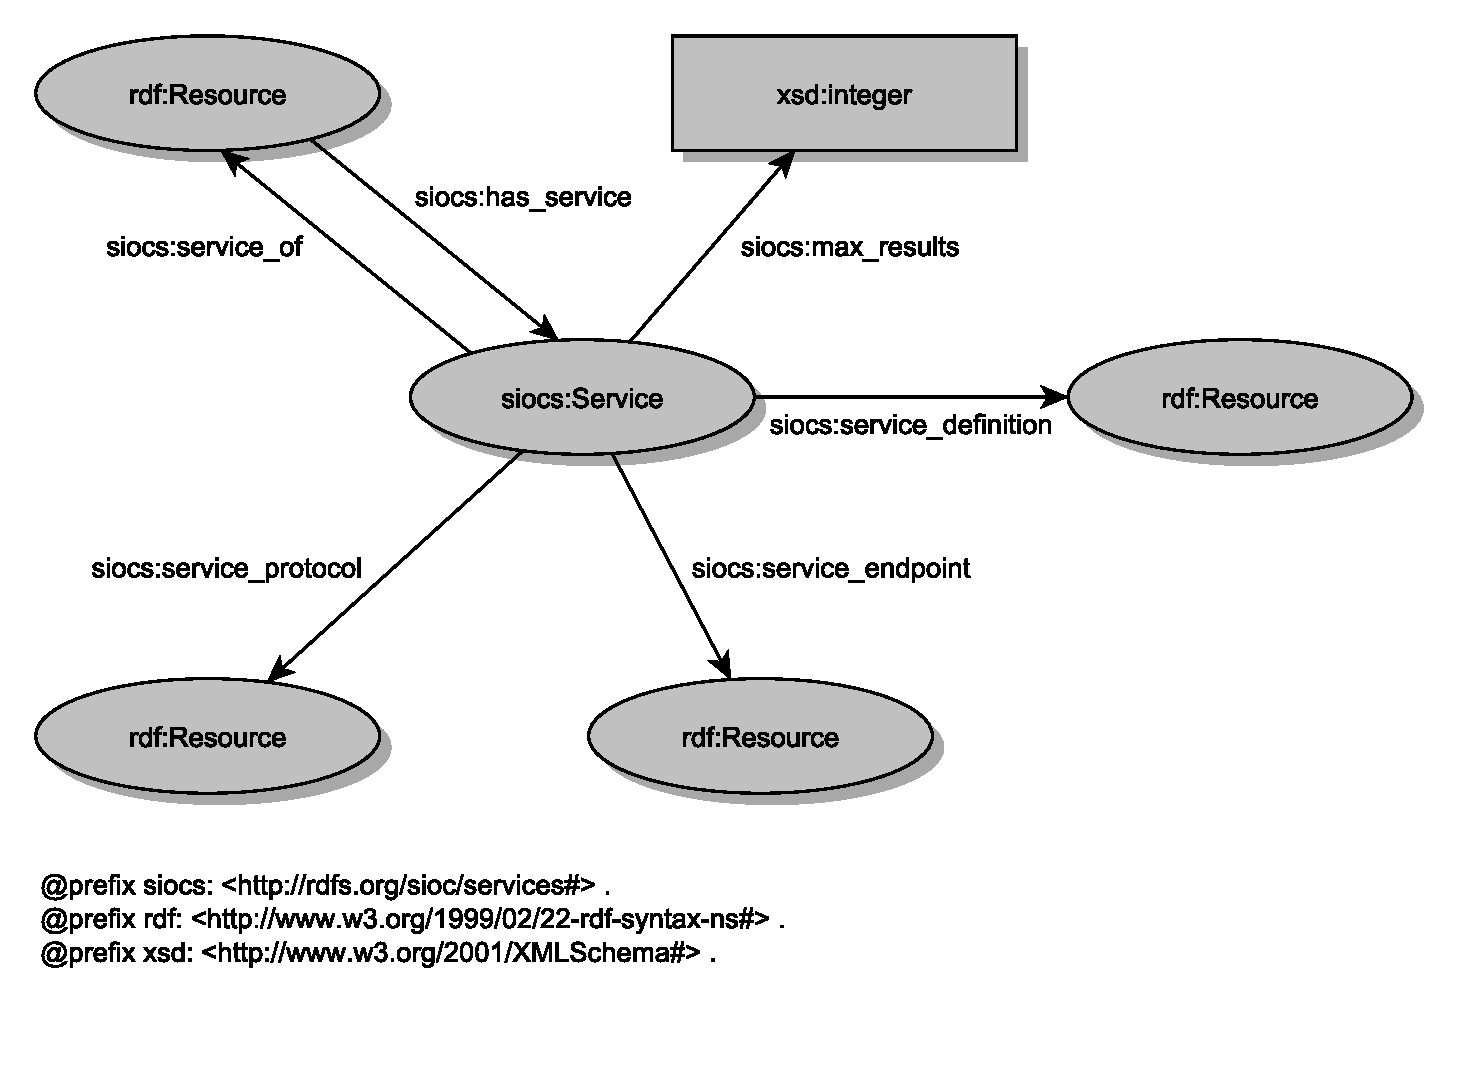
\includegraphics[
        width=0.7\textwidth,
        keepaspectratio=true
    ]{assets/images/sioc_services_ontology}
    \caption{SIOC Services Ontology}
    \label{fig:uebersicht_sioc_services}
\end{figure}

Die Eigenschaften \texttt{has\_service} und \texttt{service\_of} sind sind ideal zur Verbindung von einzelnen SIOC UserAccounts mit einem Service. Diese Verbindung hilft dabei für das stellvertretende Schreiben von Beiträgen schnell die passenden Benutzerdaten zu finden. Ebenfalls nützlich ist \texttt{max\_results}. Manche Dienste erlauben es nur eine maximale Anzahl an Ergebnissen pro Aufruf zurückgeben zu lassen. Da sich diese Anzahl über die Zeit ändern kann ist es nicht sinnvoll diese fest im Programm festzulegen, kann diese so im Nachhinein verändert werden. Für SOCC weniger interessant aber Vollständigkeit halber seien noch erwähnt \texttt{service\_protocol} zum Angeben des verwendeten Übertragungsprotokolls REST, SOAP, $\dots$) und \texttt{service\_definition} mit dem auf eine weiterführende Definition verwiesen werden kann.

% subsubsection services (end)


\subsubsection{Benutzerdaten} % (fold)
\label{ssub:benutzerdaten}

Soll ein Beitrag eines Benutzers von Google+ nach Facebook synchronisiert werden und es so aussehen, als hat er diesen Beitrag selbst auf Facebook geschrieben, sind gute Kenntnisse über alle Benutzerkonten dieser einen Person notwendig. Als erstes muss die Existenz dieser dieser Person dem System bekannt sein. Hierzu kann diese durch die Klasse Person aus der FOAF Ontologie dargestellt werden. Für ein einzelnes Benutzerkonto wurde in SIOC die Klasse die Klasse UserAccount definiert. 


% subsubsection benutzerdaten (end)


\subsubsection{Autorisierung und Authentifizierung} % (fold)
\label{ssub:autorisierung_und_authentifizierung}

Die Wahl für SIOC als Datenformat zu hat sich nach den ersten Tests als eine sehr gute Entscheidung herausgestellt. Mittels SIOC ließen die wichtigsten Daten aller untersuchten Plattformen in einer einheitlichen Form speichern. Die ersten Probleme traten erst auf, als es daran ging Daten für die Autorisierung (Feststellen ob jemand eine Handlung ausführen darf) beziehungsweise Authentifizierung (Feststellen ob jemand der ist, den er vorgibt zu sein) an den verschiedenen Programmierschnittstellen einen geeigneten Ort zu finden. Dazu musste aber erst festgestellt werden, welche verschiedenen Daten alle vorliegen können.

\medskip

\begin{description}
    \item[Username/Passwort] ist wohl eine der ersten und häufigsten Mechanismen, um den Zugriff sensibler Daten vor Dritten zu schützen. Das in Abschnitt \ref{sub:moodle_connector} beschriebene LMS Moodle, setzt zum Beispiel den Username und Password eines angemeldeten Benutzers zu Authentifizierung ein.
    
    \item[OAuth]\footnote{\url{http://oauth.net/}} stellt heutzutage den Standard der verwendeten Authentifizierungsmechanismen für hauptsächlich webbasierte API dar. Benutzer können so temporär Programmen den Zugriff auf ihre Daten erlauben und später wieder verbieten. Der aktuelle Standard stellt OAuth 2.0 dar und wird in dieser Version von den größten Seitenbetreibern wie Google, Facebook oder Microsoft eingesetzt\footnote{\url{http://en.wikipedia.org/wiki/OAuth\#List\_of\_OAuth\_service\_providers}}. Insgesamt sind für die Nutzung von OAuth vier Parameter wichtig. Für das Programm, dass Zugriff erhalten möchte sind die Parameter \emph{client\_id} und \emph{client\_secret} \cite{rfc6749}[S.\,8]. Sie weisen das Programm als autorisiert für die Benutzung der Schnittstelle aus. Soll nun beim Aufrufer einer von OAuth geschützten Funktion belegt werden ist ein sogenannter Accesstoken\cite{rfc6749}[S.\,9] nötig. Da dieser Accesstoken in der Regel nur eine bestimmte Zeit gültig ist, wird je nach Implementierung des Standards noch ein Refreshtoken mitgeliefert. Mit diesem Refreshtoken ist das Programm in der Lage ohne Zutun des Benutzers einen abgelaufen Accesstoken wieder zu aktivieren. Dies kann beliebig oft wiederholt werden, bis der Benutzer beide Token für ungültig erklärt.
    \todo[inline]{vll. noch OAuth 1.0(a) einbauen}
    
    \item[API Schlüssel] sind eine dritte Möglichkeit Programmen Zugriff auf eine API zu gewähren. Der API Schlüssel entspricht ungefähr einer Kombination von client\_id und client\_secret von OAuth. Dieser Schlüssel schaltet in der Regel nicht den Zugriff auf persönliche Daten von Benutzer frei. Hier ist noch ein weiterer Mechanismus wie die Verwendung von einem Usernamen und Passwort nötig. Die in Abschnitt \ref{sub:youtube_connector}  beschriebene Google Youtube API hierzu ein gutes Beispiel.
\end{description}

\medskip

\begin{figure}[ht]
    \centering
    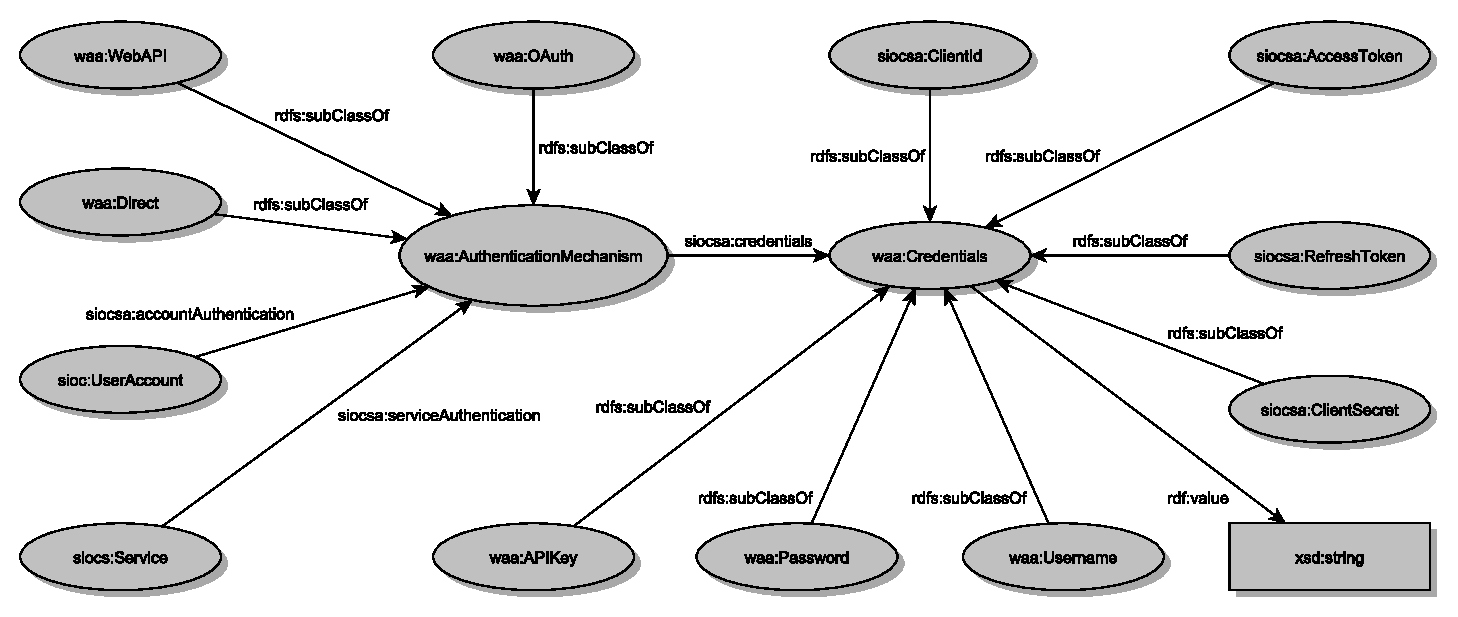
\includegraphics[
        width=\textwidth,
        keepaspectratio=true
    ]{assets/images/sioc_services_authentication}
    \caption{SIOC Services Authentication Ontology}
    \label{fig:uebersicht_sioc_services_authentication}
\end{figure}

Neben diesen drei Mechanismen wäre noch der Vollständigkeit halber die HTTP-Authentifizierung zu nennen. Hierbei handelt es ich um eine Form des Username/Passwort Verfahrens, welches auf das HTTP Protokoll aufsetzt. Für einfachen Webseiten ist dies ein unkomplizierte Art die Datei vor fremden Zugriffen zu schützten. Für aktuelle öffentliche APIs ist diese Form der Authentifizierung nicht mehr Stand der Technik.

\medskip

Die Suche nach einer bestehen Ontologie, welche zusammen mit SIOC verwendet werden könnte, gestaltete sich als sehr schwierig. Ein Großteil der Ontologien in diese Richtung befasst sich eher mit dem Thema der Autorisierung wie Zugriffssteuerungsliste wie zum Beispiel die \emph{Web Access Control List} \cite{Hollenbach2009}. Nicht desto trotz existiert auch eine Authentifizierung Ontologie. Die \emph{Authentication Ontology}\footnote{\url{http://omnivoke.kmi.open.ac.uk/authentication/}} des \emph{OmniVoke}\footnote{\url{http://omnivoke.kmi.open.ac.uk/framework/}} ist für die notwendigen Zwecke das ideale Werkzeug. 

\todo[inline]{fertig schreiben}

% subsubsection authorization (end)

% subsection konfiguration (end)

\subsection{Aufbau der SOCC} % (fold)
\label{sub:connector_aufbau}

\begin{figure}[ht]
    \centering
    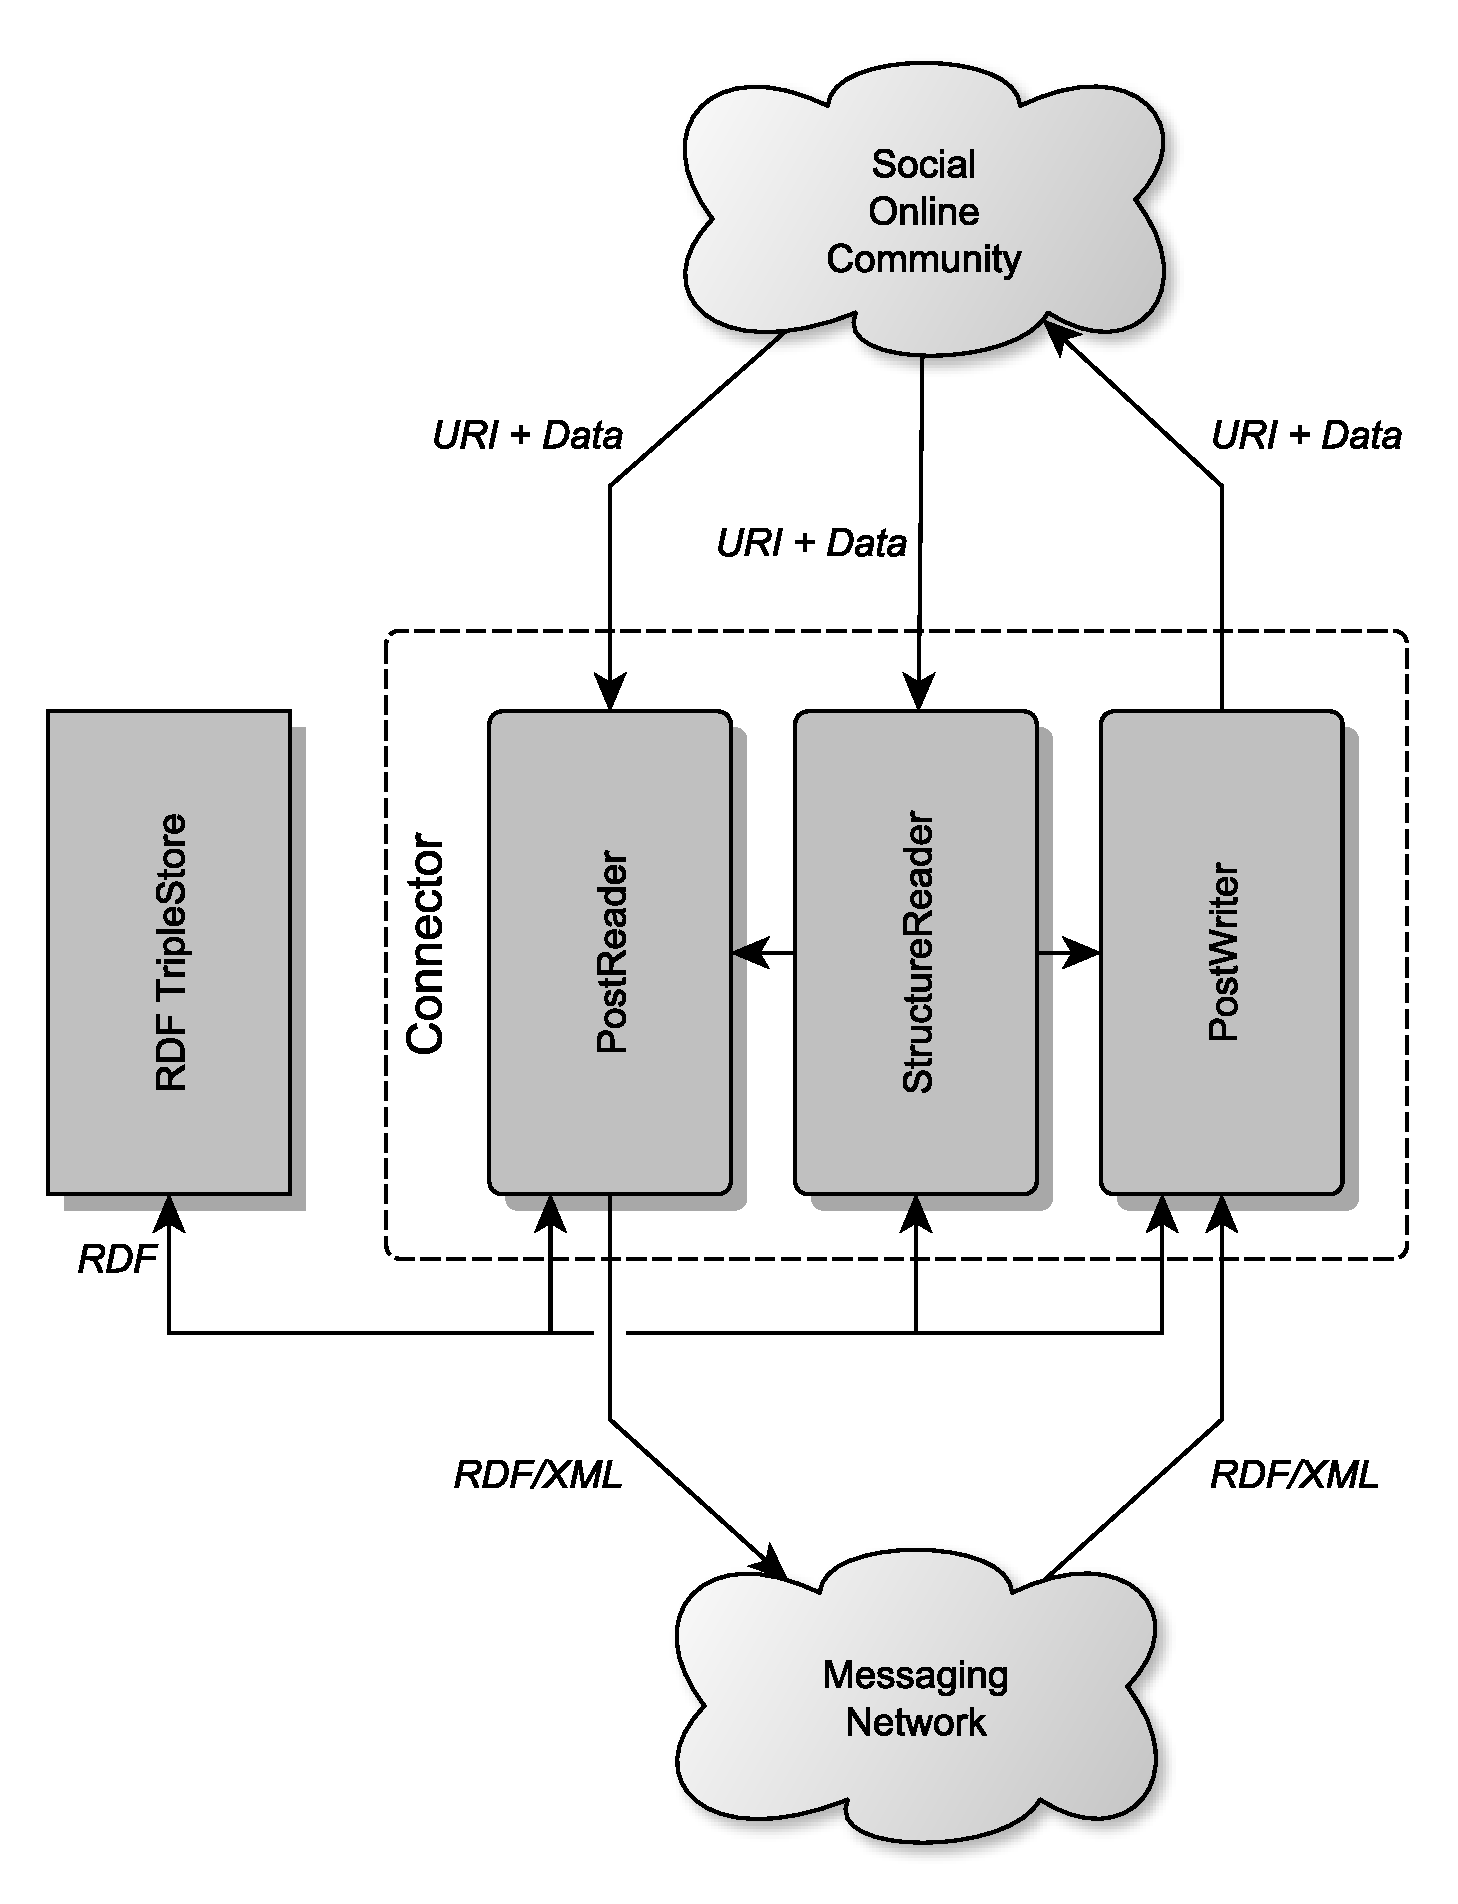
\includegraphics[
        width=0.5\textwidth,
        keepaspectratio=true
    ]{assets/images/socc_connector_overview}
    \caption{Übersicht der Komponenten der SOCC}
    \label{fig:uebersicht_socc}
\end{figure}

\subsection{Design eines Connectors} % (fold)
\label{sub:design_eines_connectors}

\begin{figure}[ht]
    \centering
    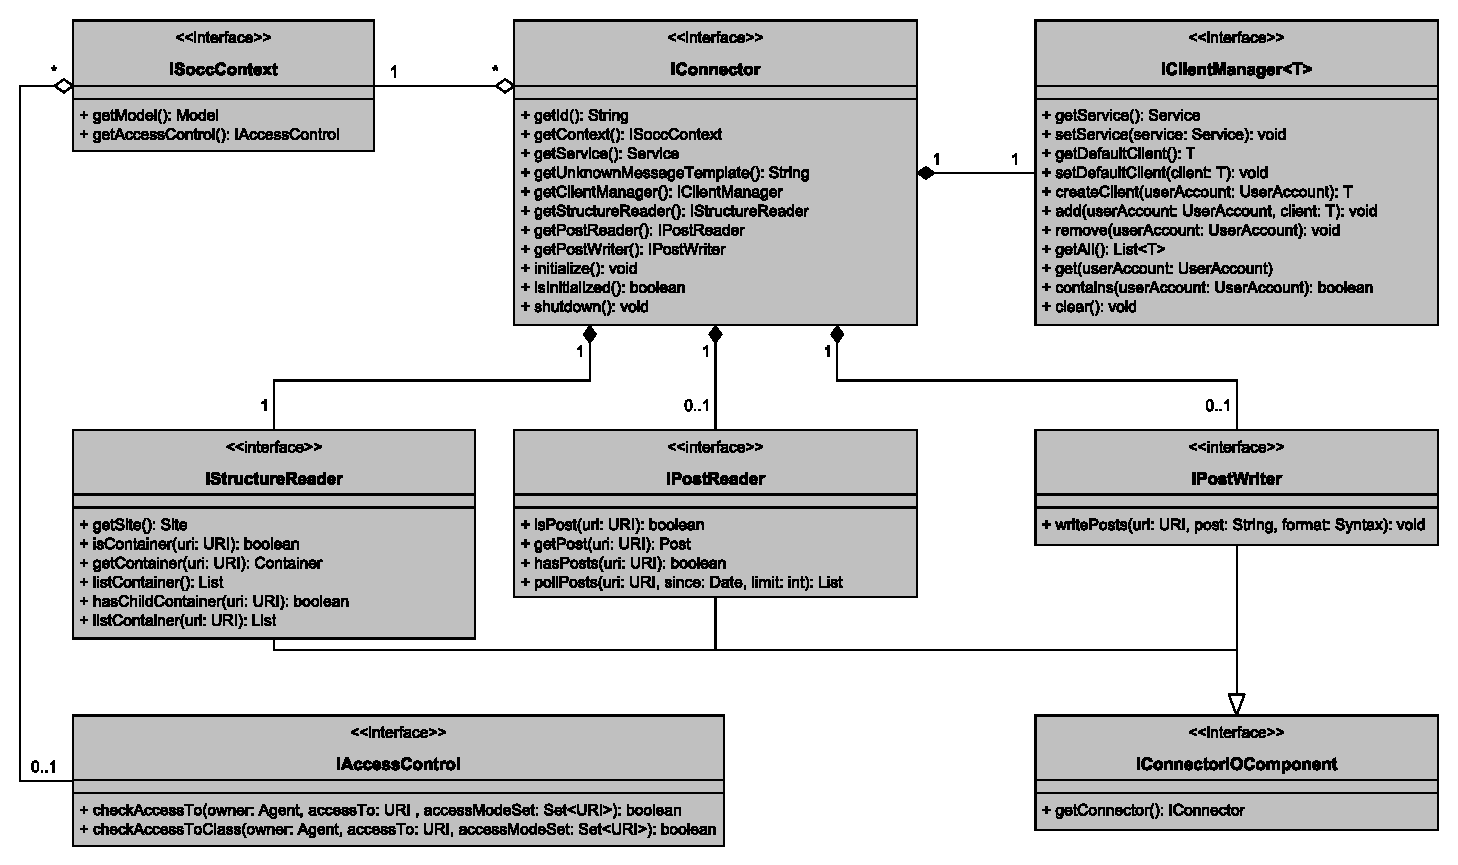
\includegraphics[
        scale=0.95,
        keepaspectratio=true,
        angle=90
    ]{assets/images/socc_uml_classdiagram}
    \caption{UML Klassendiagramm eines Connectors}
    \label{fig:connecotr_uml_classdiagram}
\end{figure}

% subsection design_eines_connectors (end)

\subsubsection{SOCC Context} % (fold)
\label{ssub:socc_context}

\begin{wrapfigure}{r}{6cm}
\centering
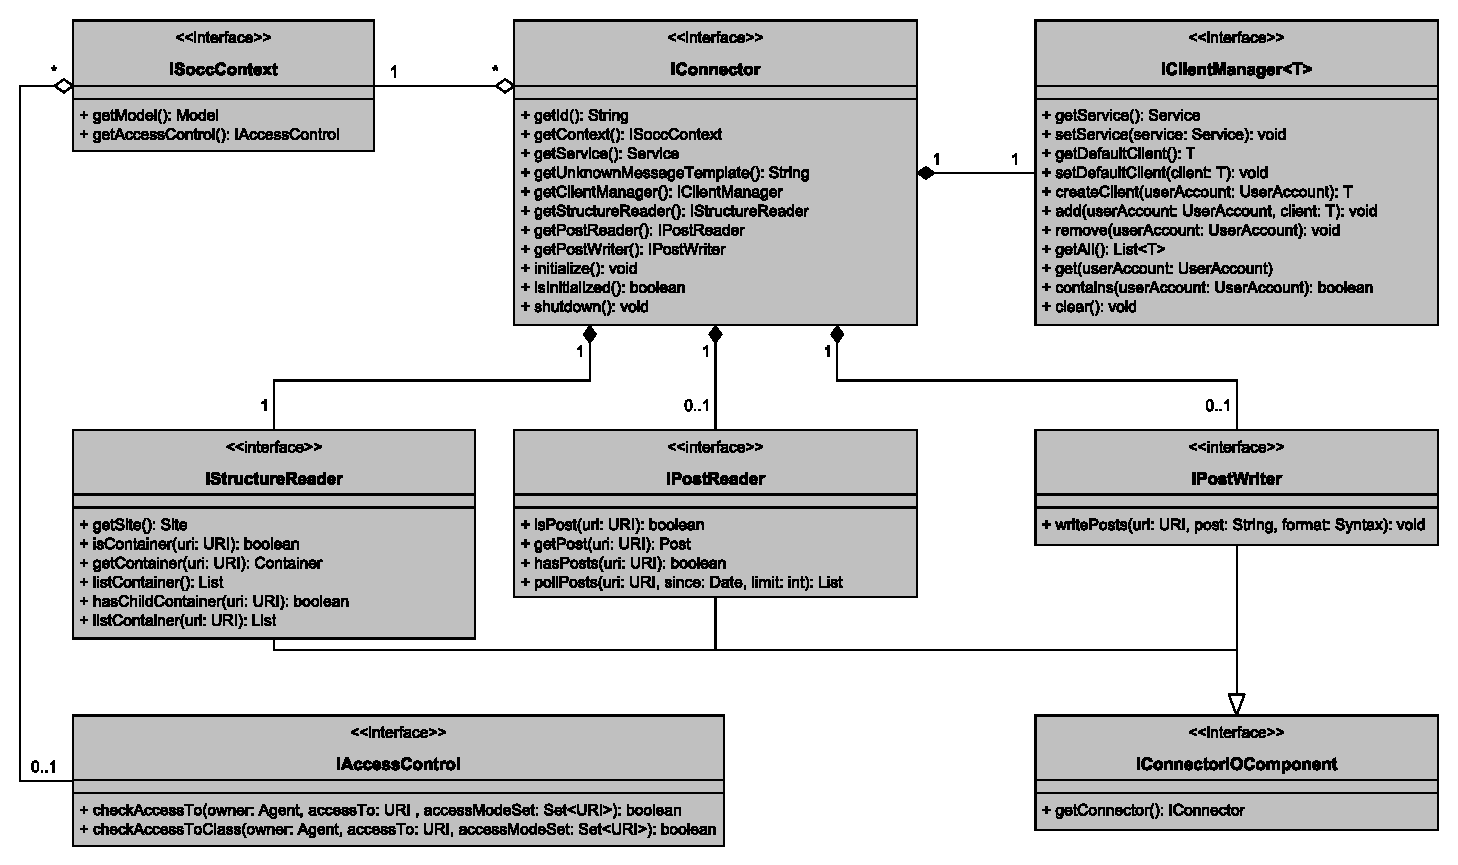
\includegraphics[
width=6cm,
keepaspectratio=true,
clip=true,
trim= 35 340 520 9
]{assets/images/socc_uml_classdiagram}
\caption{SOCC Context}
\label{fig:uml_socc_context}
\end{wrapfigure}

Text \wrapfill

% subsubsection socc_context (end)

\subsubsection{AccessControl} % (fold)
\label{ssub:accesscontrol}

\begin{figure}[ht]
\centering
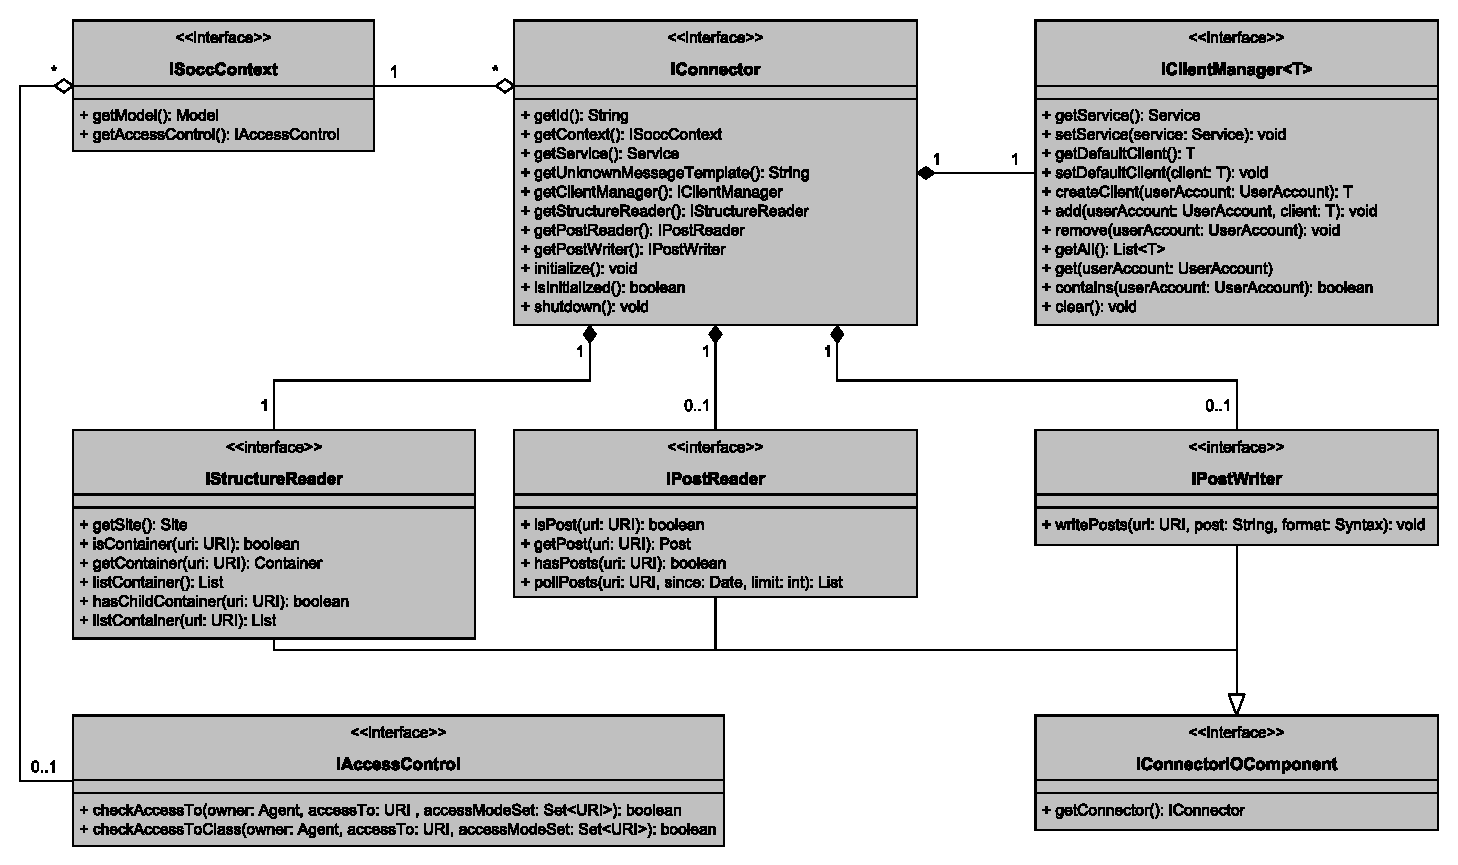
\includegraphics[
width=0.8\textwidth,
keepaspectratio=true,
clip=true,
trim= 35 8 250 340
]{assets/images/socc_uml_classdiagram}
\caption{AccessControl}
\label{fig:uml_accesscontrol}
\end{figure}

Text 

% subsubsection accesscontrol (end)


\subsubsection{ClientManager} % (fold)
\label{ssub:clientmanager}

\begin{wrapfigure}{r}{9cm}
\centering
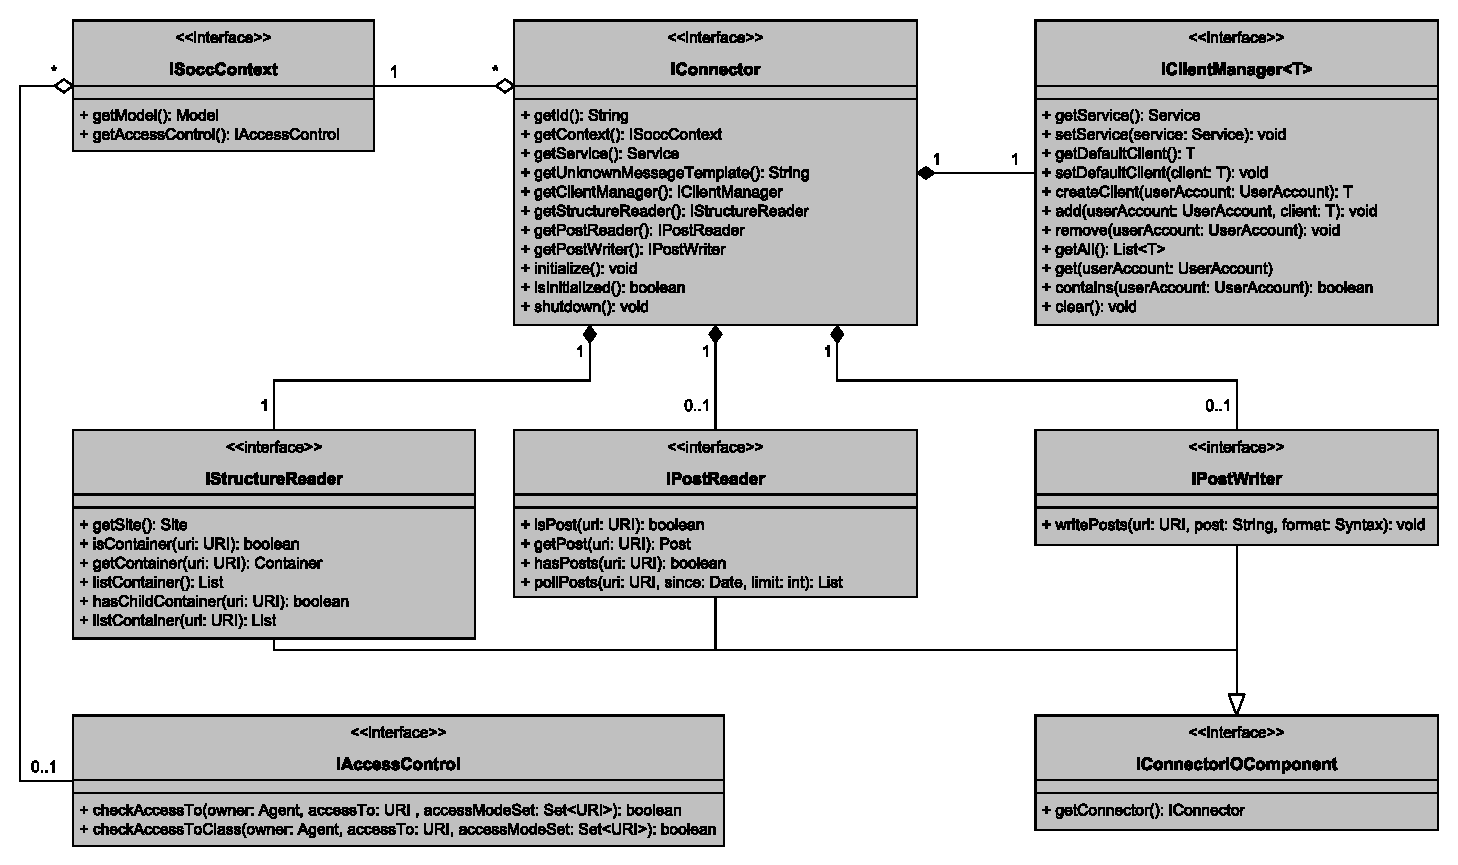
\includegraphics[
width=9cm,
keepaspectratio=true,
clip=true,
trim= 497 257 9 9
]{assets/images/socc_uml_classdiagram}
\caption{ClientManager}
\label{fig:uml_clientmanager}
\end{wrapfigure}

Der Zugriff auf eine API innerhalb eines Programms erfolgt in der Regel über eine sogenanntes Clientobjekt (kurz Client). Dieser Client erlaubt es mit den Anmeldedaten oder den Accesstoken für ein Benutzerkonto auf die Funktionen der API über verschiedene Methoden zu zugreifen. Da ein Client immer nur mit einem Benutzerkonto verknüpft ist und von diesen eine große Anzahl verwaltet werden müssen, enthält jeder Connector einen ClientManager. Der interne Aufbau eines Client ist dabei stark von der verwendeten API abhängig und arbeitet mit dem Connector zusammen für den er geschrieben wurde. Für alle benutzerunabhängigen Daten erhält der ClientManager ein wie Abschnitt \ref{ssub:services} beschriebenes Serviceobjekt. Ein neuer Client kann dann durch den Aufruf der Methode \lstinline[language=java]{createClient($\dots$)} erstellt werden. Als Parameter wird der Methode ein Benutzerkonto in Form eines SIOC UserAccounts übergeben. Sind alle erforderlichen Autorisierung- und Authentifizierungsinformation aus Abschnitt \ref{ssub:autorisierung_und_authentifizierung} vorhanden, wird ein neuer Client erzeugt und zurück gegeben. Dieser Client wird aber dadurch nicht automatisch vom ClientManager verwaltet. Hierzu muss der im vorherigen erzeugte Client durch den Aufruf von \lstinline[language=java]{add(userAccount: UserAccount, client: T )} dauerhaft mit den angegeben UserAccount verknüpft und intern gespeichert. Wichtig ist hierbei, dass die Eigenschaften \texttt{accountName} und \texttt{accountServiceHomepage} des UserAccount Objekts gesetzt sind. Aus diesen wird ein eindeutiger Schlüssel generiert der zur Zuordnung von UserAccount und Client innerhalb des ClientManagers dient. Dieser Zwischenschritt ist einer verbesserten Abstraktion bei der späteren Implementierung geschuldet, da nur die Methode \lstinline[language=java]{createClient} stark von der verwendeten API Bibliothek abhängt. Des weiteren stehen noch Methoden \lstinline[language=java]{remove(userAccount: UserAccount)} zum Entfernen und \lstinline[language=java]{get(userAccount: UserAccount)} Holen von Clients, sowie \lstinline[language=java]{contains(userAccount: UserAccount)} für Tests ob ein Client zu einem UserAccount existiert. Sollen zum Beispiel am Ende der Laufzeit des Programms alle erzeugten Clients auf einmal abgemeldet und gelöscht werden, kann dies über die Methode \lstinline[language=java]{clear()} erfolgen. Der ClientManager verwaltet ebenfalls den Client für den in Abschnitt \ref{ssub:connector_config_ontologie} angesprochenen Defaultuser. Dieser Defaultclient genannte Client kann über die Methode  \lstinline[language=java]{setDefaultClient(client: T)} gesetzt und durch \lstinline[language=java]{getDefaultClient()} jederzeit wieder abgerufen werden. 

% subsubsection clientmanager (end)

\subsubsection{StructureReader} % (fold)
\label{ssub:structurereader}

\begin{wrapfigure}[10]{r}{9cm}
    \centering
    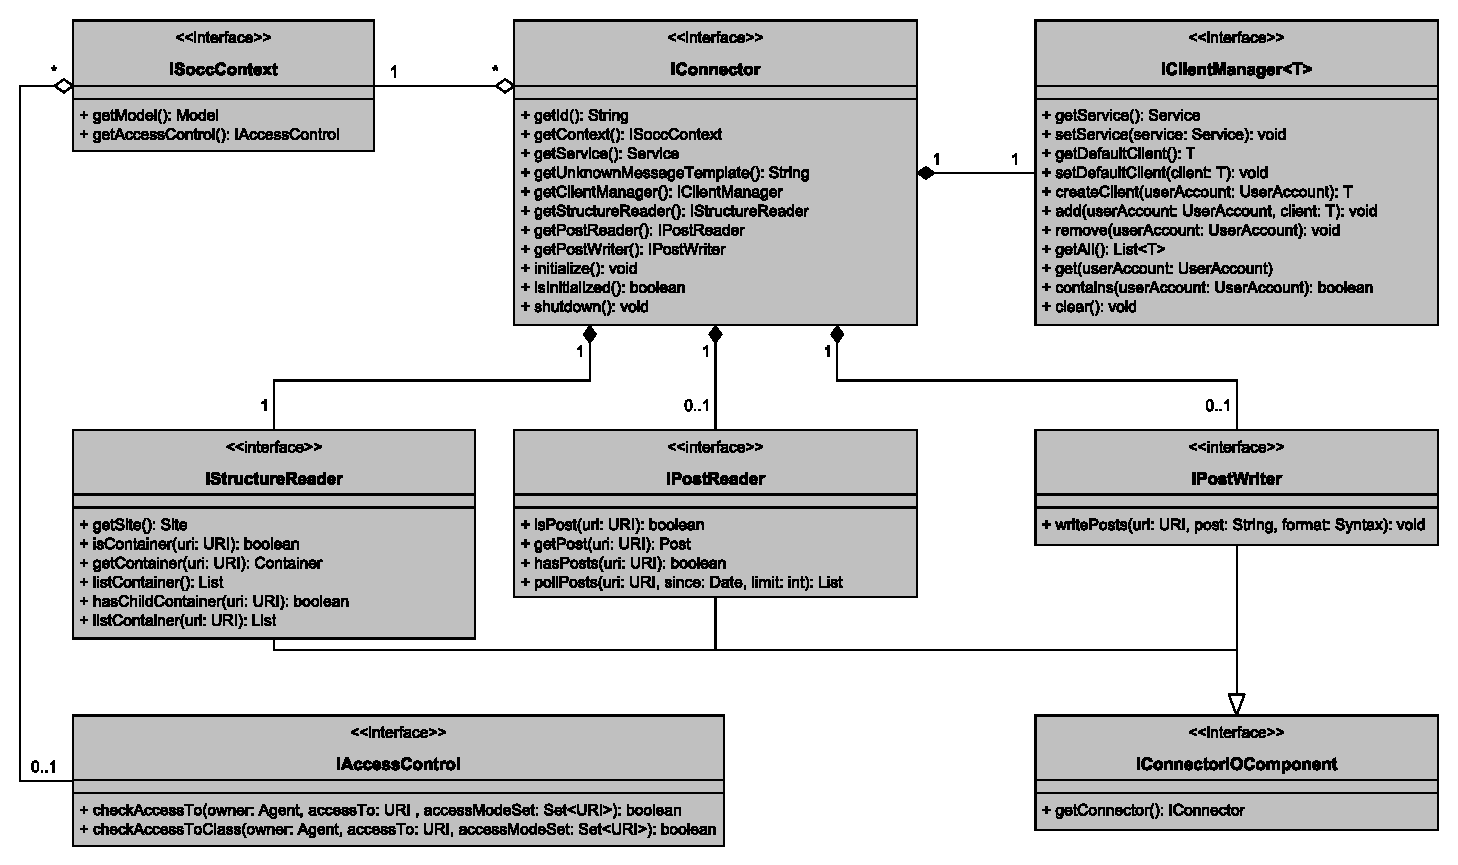
\includegraphics[
        width=9cm,
        keepaspectratio=true,
        clip=true,
        trim= 20 118 456 206
    ]
    {assets/images/socc_uml_classdiagram}
    \caption{StructurReader}
    \label{fig:uml_structure_reader}
\end{wrapfigure}
Um auf Informationen über die Struktur von Foren, sozialen Netzwerken und so weiter im SIOC Format zugreifen zu können, implementiert jeder Connector dazu einen StructureReader. Die Struktur lässt sich, wie im Abschnitt \ref{sec:social_online_community_connectors} vorgestellt, durch die SIOC Klassen \emph{Site} und \emph{Container} (und Unterklassen davon) beschrieben. Um auf diese Struktur zugreifen zu können, enthält die StructureReader Schnittstelle mehrere Methode (Siehe Abbildung \ref{fig:uml_structure_reader}). \wrapfill

\begin{description}
    \item[\texttt{getSite()}] ist eine Methode, welche die Beschreibung einer Seite (Forum, Blog, soziales Netzwerk) als SIOC Site Objekt zurücklieft. Dies wird relativ häufig um die Zugehörigkeit einiger Objekte durch einen Link zu dieser Seite zu verdeutlichen. Dies kann bei einigen APIs nützlich sein, da dort manchmal keine Information zum \emph{Container} eines Beitrags mitgeliefert werden, über den man sonst eine Beziehung zwischen Seite und Beitrag herstellen könnte.

    \item[\texttt{getContainer(URI)}] ist dazu gedacht die Information eines einzelnen Containers erhalten der sich hinter eine URI verbirgt.

    \item[\texttt{listContainer(...)}] sind Methoden welche für den die Auflisten aller Container einer Seite zur Verfügung stehen. Die Methode ohne Parameter listet alle Container auf der ersten Ebene auf. Dies könnten zum Beispiel alle Kurse auf einen Canvas LMS Seite oder alle Gruppen auf Facebook sein. Die zweite Methode mit URI Parameter gibt eine Liste alle Container, welche den Container hinter der übergeben URI als Elternteil haben, zurück. Als Beispiel wären alle Themen innerhalb eines Forums zu nennen.

    \item[\texttt{hasChildContainer(URI)}] überprüft ob der Container hinter einer URI überhaupt weitere Container als Kinder besitzt. Diese Methode wird dazu eingesetzt, um vorab zu testen, ob der Aufruf von \texttt{listContainer(URI)} das gewünschte Ergebnis liefert oder ein Fehler auftritt. 
\end{description}

% subsubsection structurereader (end)

\subsubsection{PostReader} % (fold)
\label{ssub:postreader}

\begin{wrapfigure}{r}{9cm}
\centering
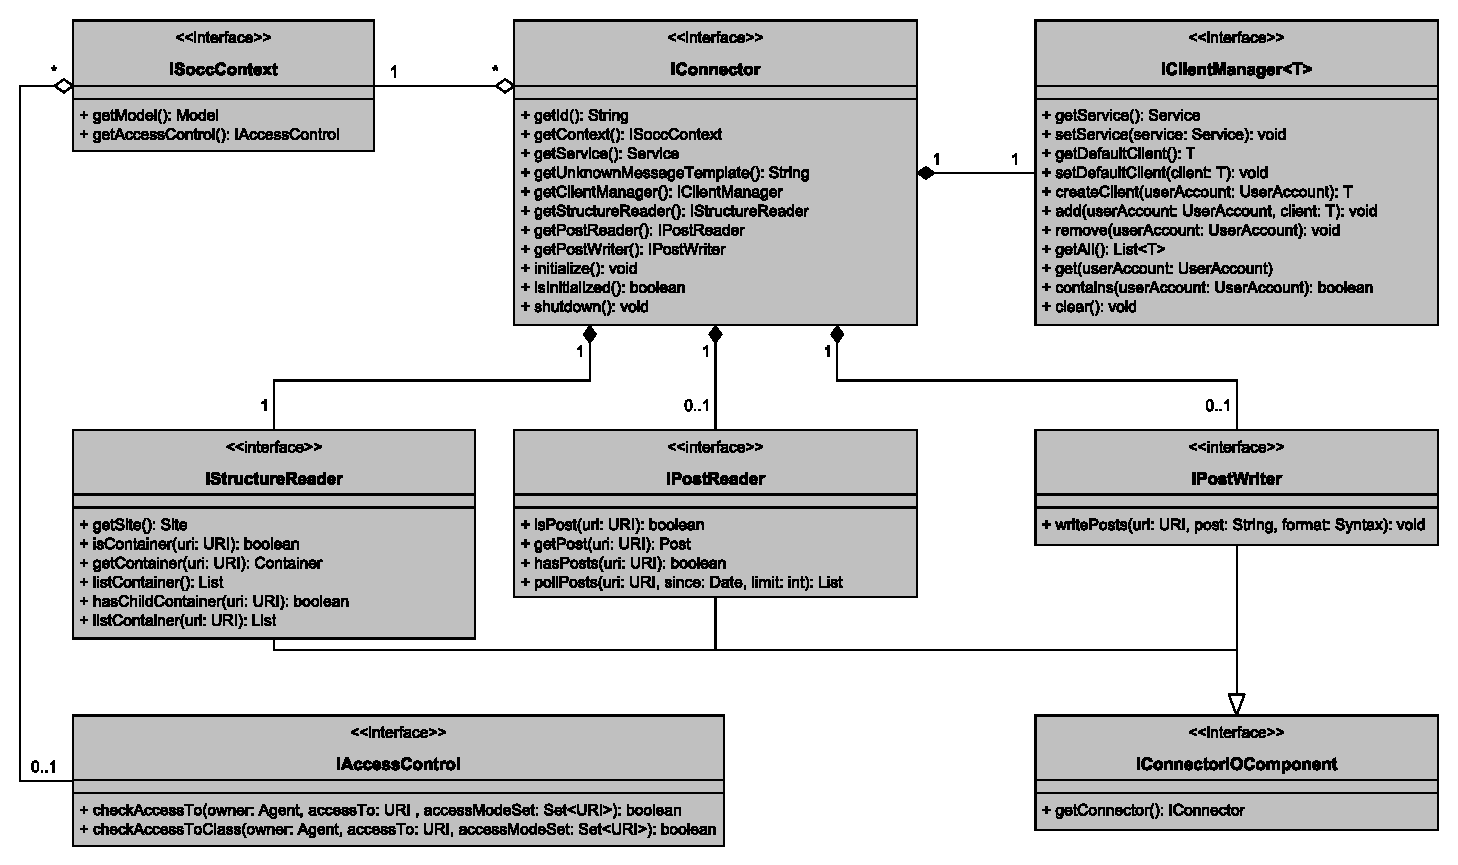
\includegraphics[
width=9cm,
keepaspectratio=true,
clip=true,
trim= 243 137 255 206
]{assets/images/socc_uml_classdiagram}
\caption{PostReader}
\label{fig:uml_post_reader}
\end{wrapfigure}

Der \texttt{PostReader} dient als Schnittstelle, um auf geschriebene Beitrage innerhalb eines Containers oder die Kommentare auf eines Beitrags zuzugreifen. Die Methode \texttt{hasPosts(URI)} ist nur zur Überprüfung ob ein Container oder ein Beitrag hinter einer URI weiter Beiträge enthält die gelesen werden können. Um einen einzelnen Beitrag anhand seiner URI lesen zu können kann die Methode \texttt{getPost(URI)}  genutzt werden. Sei liefert dann den Beitrag SIOC Post Objekt zurück beziehungsweise einen Fehler, falls der Beitrag nicht mit diesem Connector gelesen werden kann. Die wichtigste Methode dahingegen ist \texttt{pollPosts(URI, Date, int)}. Insgesamt können dieser Methode drei Parameter übergeben werden. Der Erste ist eine URI die den Ort angibt von der alle Beiträge gelesen werden können. Mit dem zweiten Parameter kann ein Zeitpunkt angegeben werden, ab dem ein zu lesender Beitrag geschrieben sein muss. Alle Beiträge die vor diesem Zeitpunkt erstellt wurden, werden nicht zurück gegeben. Der letzte Parameter gibt eine obere Schranke an wie viele Beiträge maximal pro Aufruf dieser Methode gelesen werden dürfen.

% subsubsection postreader (end)

\subsubsection{PostWriter} % (fold)
\label{ssub:postwriter}

In Abbildung \ref{fig:postwriter_sequenzdiagramm} ist ein Sequenzdiagramm der PostWriter Komponente zu sehen. Dort ist visualisiert, welche Schritte für das stellvertretende Schreiben von Beiträgen eines Benutzers unternommen werden müssen. Soll nun ein Beitrag in einer SOC geschrieben werden, wird die Methode \texttt{writePost(URI, String, Syntax)} mit dem Zielort als URI, dem Beitrag als serialisiertes RDF Objekt und dem verwendeten Serialisierungsformates aufgerufen. Begonnen wird damit, dass als erstes nach einem UserAccount für den Service des aktuellen Connectors des Beitragautors gesucht. Im Idealfall befindet sich für den UserAccount des Beitragsautors ein Link zu seiner FOAF Person und von ein weiterer Link zum UserAccount für den aktuellen Service. Mit diesem UserAccount kann dann vom ClientManager ein Clientobjekt für die verwendete API angefordert werden. Sollte die Suche negativ verlaufen, steht der Defaultclient zur Verfügung. Mit diesem Client, ob mit der des Autors oder dem Defaultclient, wird im letzten Schritt der Beitrag im von der API verwendeten Format in die SOC geschrieben.
\begin{figure}[ht]
\centering
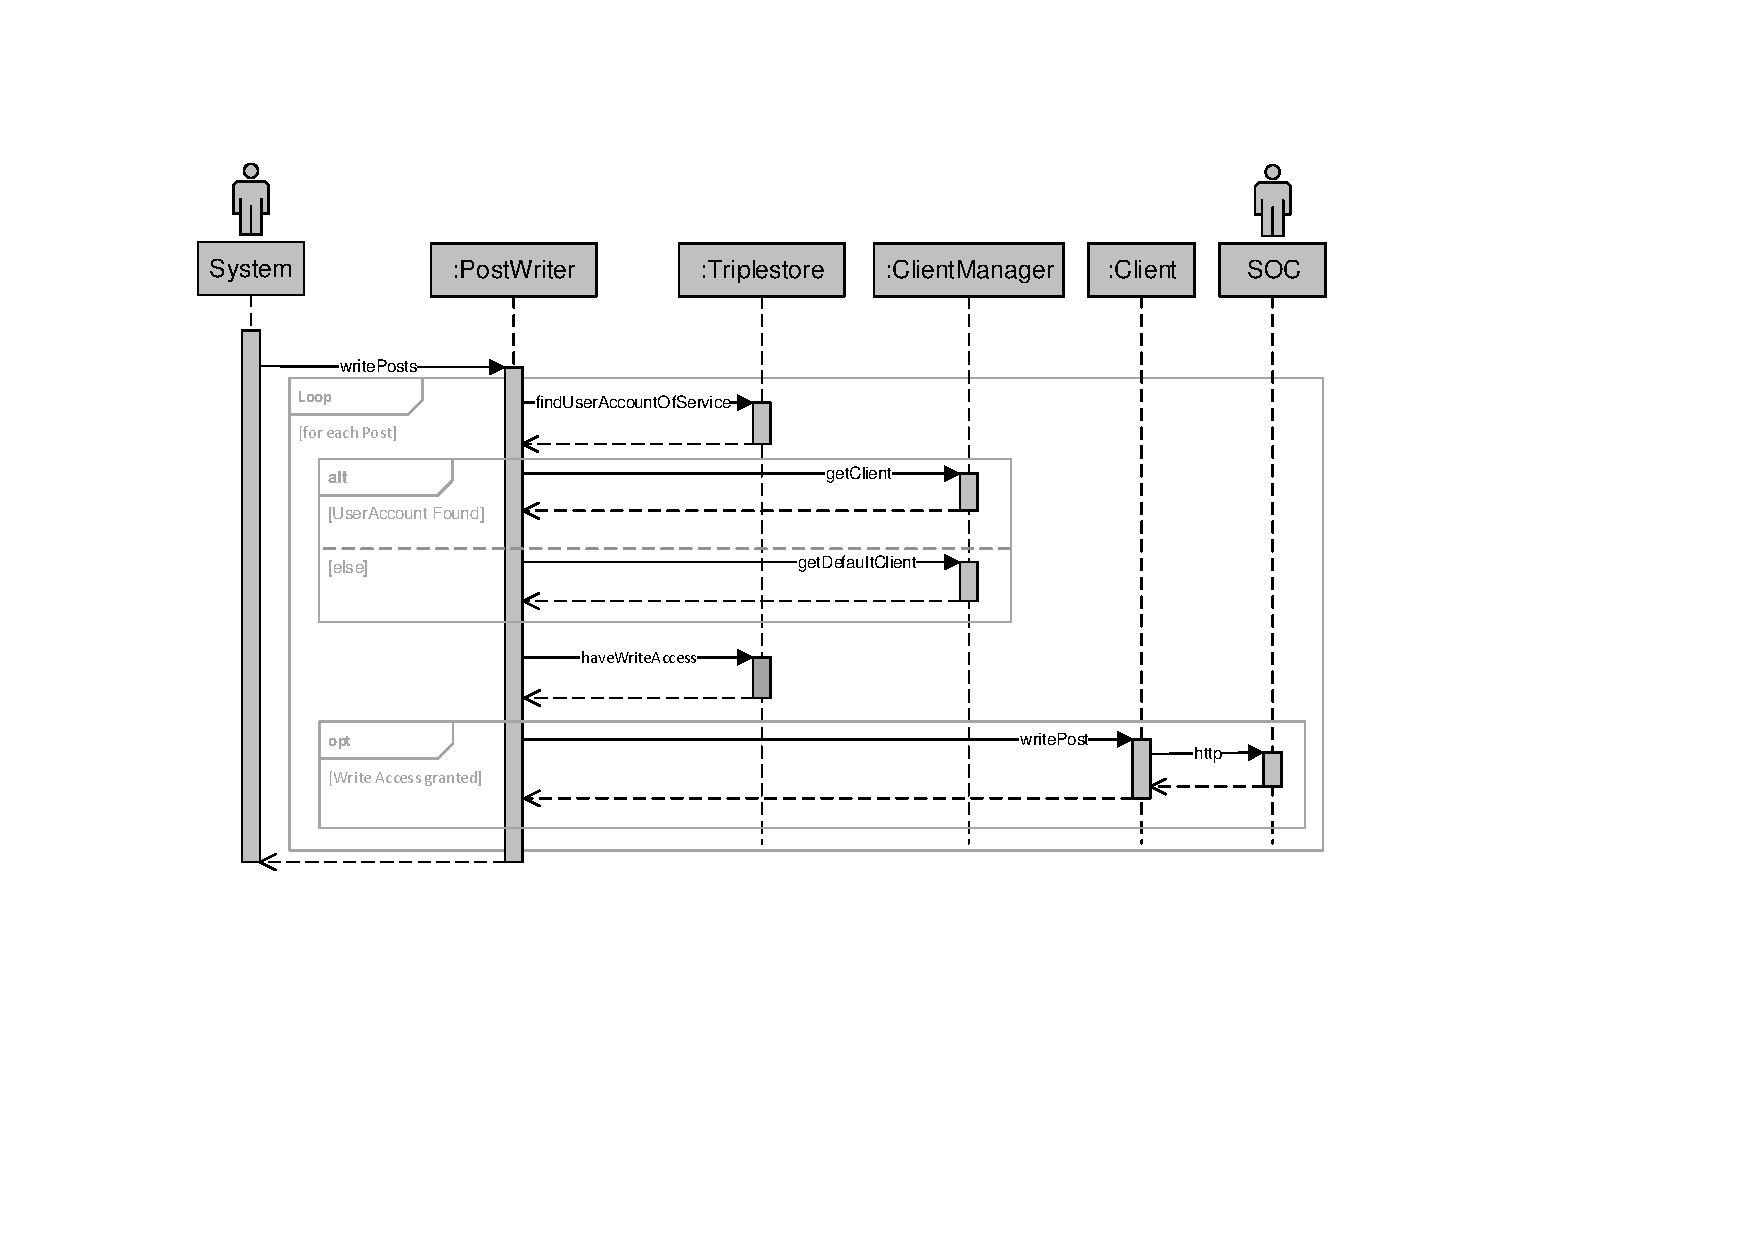
\includegraphics[
width=\textwidth,
keepaspectratio=true,
clip=true,
trim= 90 200 220 75
]{assets/images/postwriter_sequencediagram}
\caption{PostWriter Sequenzdiagramm}
\label{fig:postwriter_sequenzdiagramm}
\end{figure}

% subsubsection postwriter (end)

% subsection connector_aufbau (end)

% section social_online_community_connectors (end)

\section{SOCC-Camel} % (fold)
\label{sec:socc_camel}

\begin{figure}[ht]
     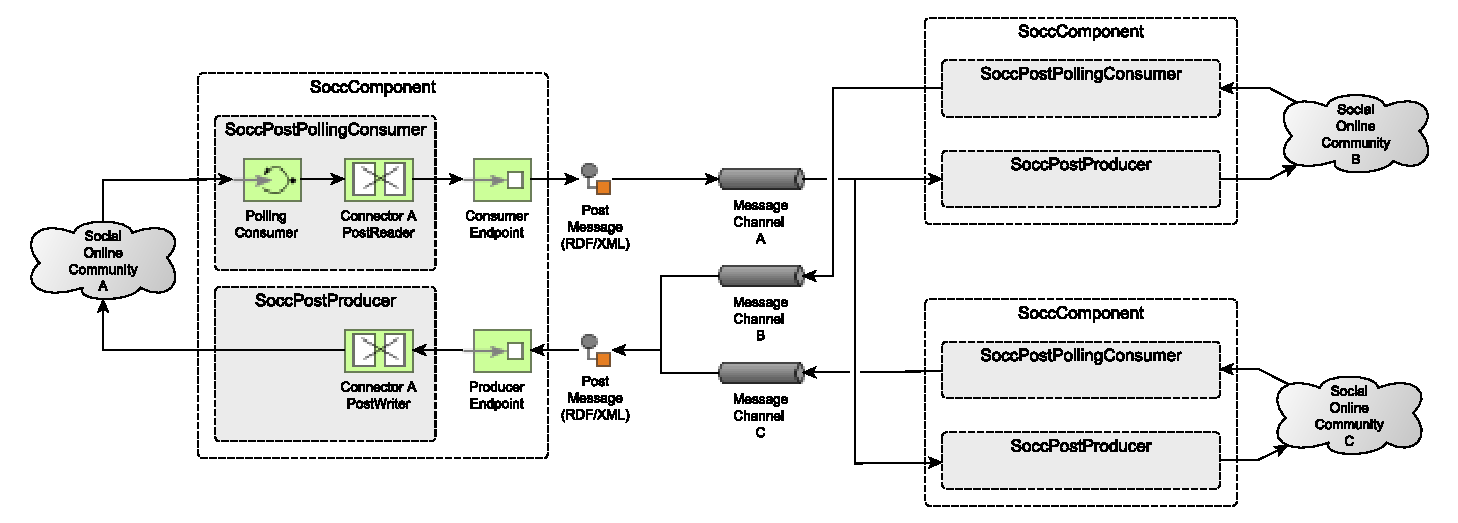
\includegraphics[
        width=\textwidth,
        keepaspectratio=true
    ]{assets/images/socc_camel_overview}
    \caption{Übersicht des Apache Camel Moduls Socc-Camel}
    \label{fig:uebersicht_socc_camel}
\end{figure}

\subsection{SoccComponent} % (fold)
\label{sub:socccomponent}

% subsection socccomponent (end)

\subsection{SoccPostPollingConsumer} % (fold)
\label{sub:soccpostpollingconsumer}

% subsection soccpostpollingconsumer (end)

\subsection{SoccPostProducer} % (fold)
\label{sub:soccpostproducer}

% subsection soccpostproducer (end)

% section socc_camel (end)

% chapter eigener_ansatz (end)
